\documentclass[12pt,a4paper]{article}
\usepackage[margin=2cm]{geometry}
\usepackage{amsmath,amssymb,amsfonts}
\usepackage{tikz}
\usetikzlibrary{patterns,arrows.meta,calc,angles,quotes,decorations.markings}
\usepackage{enumitem}
\usepackage{xcolor}
\usepackage{fancyhdr}
\usepackage{titlesec}
\usepackage{tcolorbox}
\usepackage{multicol}

\definecolor{examblue}{RGB}{0,51,102}
\definecolor{examred}{RGB}{153,0,0}
\definecolor{solutionbox}{RGB}{240,248,255}

\pagestyle{fancy}
\fancyhf{}
\rhead{\textbf{Mechanics Module}}
\lhead{\textbf{Ultimate Past Paper 2}}
\rfoot{Page \thepage}
\renewcommand{\headrulewidth}{1.5pt}
\renewcommand{\footrulewidth}{0.5pt}

\titleformat{\section}{\Large\bfseries\color{examblue}}{}{0em}{}[\titlerule]
\titleformat{\subsection}{\large\bfseries\color{examred}}{}{0em}{}

\newtcolorbox{questionbox}[1][]{
    colback=solutionbox, colframe=examblue, boxrule=1.5pt, arc=3mm, #1
}
\newtcolorbox{mcqbox}{
    colback=white, colframe=examred, boxrule=1pt, arc=2mm, left=5mm, right=5mm
}

\begin{document}

\begin{titlepage}
    \centering
    \vspace*{2cm}
    {\Huge\bfseries\color{examblue}MECHANICS MODULE}\par
    \vspace{0.5cm}
    {\Large\bfseries ULTIMATE PAST PAPER 2}\par
    \vspace{1.5cm}
    {\large Examination Period: May (Main)}\par
    \vspace{0.5cm}
    \rule{\linewidth}{2pt}\par
    \vspace{1cm}
    {\Large Time Allowed: \textbf{2 hours}}\par
    \vspace{0.5cm}
    {\Large Total Marks: \textbf{100} (40\% of Module)}\par
    \vspace{1.5cm}
    \rule{\linewidth}{1pt}\par
    \vspace{1cm}
    {\large\bfseries INSTRUCTIONS TO CANDIDATES}\par
    \vspace{0.5cm}
    \begin{minipage}{0.8\linewidth}
        \begin{enumerate}[label=\textbf{\arabic*.},leftmargin=*]
            \item Answer ALL questions
            \item Section A: 6 Short Multiple Choice Questions (60 marks)
            \item Section B: 2 Long Multiple Choice Questions (40 marks)
            \item All questions are compulsory and extremely challenging
            \item Calculators permitted (must not store text)
        \end{enumerate}
    \end{minipage}
    \vfill
    {\small University of Birmingham - School of Engineering}\par
\end{titlepage}

\newpage
\section*{SECTION A: SHORT MULTIPLE CHOICE QUESTIONS (60 Marks)}
{\large\itshape Answer all 6 questions. Each question carries 10 marks.}

\vspace{0.5cm}

\begin{questionbox}
\subsection*{Question A1: Indeterminate Truss with Support Settlement [10 marks]}

The pin-jointed truss shown has a support settlement at $C$ of $\delta_C = 8\,\text{mm}$ downward.
All members have $AE = 45,000\,\text{kN}$. The truss carries vertical loads of $60\,\text{kN}$ at $B$ 
and $40\,\text{kN}$ at $D$.

\begin{center}
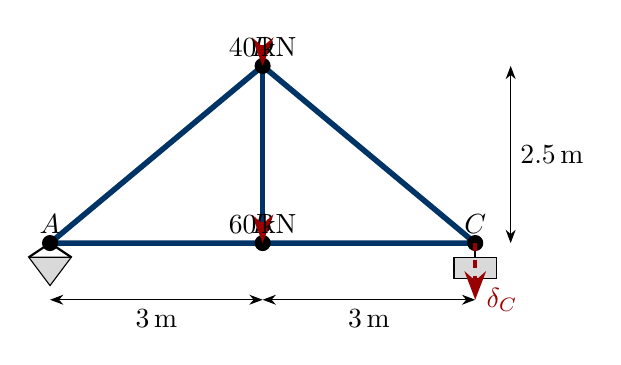
\begin{tikzpicture}[scale=0.9,>=Stealth]
    \coordinate (A) at (0,0);
    \coordinate (B) at (3,0);
    \coordinate (C) at (6,0);
    \coordinate (D) at (3,2.5);
    
    \draw[thick,examblue,line width=2pt] (A)--(B)--(C)--(D)--(A)--(D);
    \draw[thick,examblue,line width=2pt] (B)--(D);
    
    \foreach \pt/\lbl in {A/A,B/B,C/C,D/D}
        \filldraw[black] (\pt) circle (3pt) node[above] {$\lbl$};
    
    % Supports
    \draw[fill=gray!30] (A)++(-0.3,-0.2)--++(0.6,0)--++(-0.3,-0.4)--cycle;
    \draw[thick] (A)++(-0.3,-0.2)--(A)--++(0.3,-0.2);
    
    \draw[fill=gray!30] (C)++(-0.3,-0.5) rectangle ++(0.6,0.3);
    \draw[thick] (C)--++(0,-0.2);
    \draw[->,examred,dashed,ultra thick] (C) -- ++(0,-0.8) node[right] {$\delta_C$};
    
    % Loads
    \draw[->,examred,ultra thick] (B)++(0,0.3)--(B);
    \node[above] at (B) {$60\,\text{kN}$};
    \draw[->,examred,ultra thick] (D)++(0,0.3)--(D);
    \node[above] at (D) {$40\,\text{kN}$};
    
    % Dimensions
    \draw[<->] (0,-0.8)--node[below]{$3\,\text{m}$}(3,-0.8);
    \draw[<->] (3,-0.8)--node[below]{$3\,\text{m}$}(6,-0.8);
    \draw[<->] (6.5,0)--node[right]{$2.5\,\text{m}$}(6.5,2.5);
\end{tikzpicture}
\end{center}

Using the flexibility method, determine the force in member $BD$.

\begin{mcqbox}
\begin{enumerate}[label=(\Alph*),leftmargin=*]
    \item $+28.4\,\text{kN}$ (Tension)
    \item $-35.7\,\text{kN}$ (Compression)
    \item $+42.1\,\text{kN}$ (Tension)
    \item $-31.9\,\text{kN}$ (Compression)
    \item $+38.6\,\text{kN}$ (Tension)
\end{enumerate}
\end{mcqbox}
\end{questionbox}

\begin{questionbox}
\subsection*{Question A2: Unsymmetrical Bending of Z-Section [10 marks]}

The Z-section beam shown is subjected to a bending moment $M = 25\,\text{kNm}$ applied 
at an angle $\theta = 30^\circ$ to the horizontal axis. All dimensions in mm.

\begin{center}
\begin{tikzpicture}[scale=0.6,>=Stealth]
    % Z section
    \draw[thick,examblue,line width=2pt] (0,0)--(6,0)--(6,0.5)--(1.5,0.5)--(1.5,5.5)--(6,5.5)--(6,6)--(0,6)--(0,5.5)--(4.5,5.5)--(4.5,0.5)--(0,0.5)--cycle;
    
    % Axes
    \draw[->,examred,ultra thick] (3,3)--(5,3) node[right] {$x$};
    \draw[->,examred,ultra thick] (3,3)--(3,5) node[above] {$y$};
    
    % Moment vector
    \draw[->,examblue,ultra thick] (7,3) arc (0:30:1);
    \node[right] at (8,3.3) {$M$};
    \pic["$\theta=30^\circ$",draw,angle radius=0.6cm] {angle={(5,3)--(3,3)--(3.9,3.5)}};
    
    % Dimensions
    \draw[<->] (0,-0.5)--node[below]{$150$}(6,-0.5);
    \draw[<->] (-0.5,0)--node[left]{$600$}(-0.5,6);
    \draw[<->] (6.5,0.5)--node[right]{$50$}(6.5,5.5);
\end{tikzpicture}
\end{center}

Given $I_{xx} = 285\times10^6\,\text{mm}^4$, $I_{yy} = 42\times10^6\,\text{mm}^4$, $I_{xy} = -68\times10^6\,\text{mm}^4$,
determine the maximum tensile stress in the section.

\begin{mcqbox}
\begin{enumerate}[label=(\Alph*),leftmargin=*]
    \item $127.3\,\text{MPa}$
    \item $142.8\,\text{MPa}$
    \item $98.6\,\text{MPa}$
    \item $156.4\,\text{MPa}$
    \item $118.9\,\text{MPa}$
\end{enumerate}
\end{mcqbox}
\end{questionbox}

\begin{questionbox}
\subsection*{Question A3: Curved Beam Stress Analysis [10 marks]}

The curved beam with rectangular cross-section ($b=50\,\text{mm}$, $h=100\,\text{mm}$) has 
inner radius $r_i = 150\,\text{mm}$ and carries a bending moment $M = 12\,\text{kNm}$ 
that tends to straighten the beam.

\begin{center}
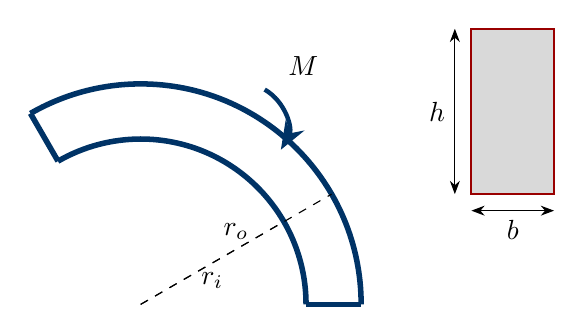
\begin{tikzpicture}[scale=0.7,>=Stealth]
    % Curved beam
    \draw[thick,examblue,line width=2pt] (0:3) arc (0:120:3);
    \draw[thick,examblue,line width=2pt] (0:4) arc (0:120:4);
    \draw[thick,examblue,line width=2pt] (0:3)--(0:4);
    \draw[thick,examblue,line width=2pt] (120:3)--(120:4);
    
    % Cross-section detail
    \begin{scope}[xshift=6cm,yshift=2cm]
        \draw[thick,examred,fill=gray!30] (0,0) rectangle (1.5,3);
        \draw[<->] (-0.3,0)--node[left]{$h$}(-0.3,3);
        \draw[<->] (0,-0.3)--node[below]{$b$}(1.5,-0.3);
    \end{scope}
    
    % Moment
    \draw[->,examblue,ultra thick] (60:4.5) arc (60:-30:0.8);
    \node[right] at (60:5) {$M$};
    
    % Radii
    \draw[dashed] (0,0)--(30:3) node[midway,below]{$r_i$};
    \draw[dashed] (0,0)--(30:4) node[midway,above]{$r_o$};
\end{tikzpicture}
\end{center}

Using Winkler-Bach theory for curved beams, determine the maximum compressive stress 
(at the inner fiber).

\begin{mcqbox}
\begin{enumerate}[label=(\Alph*),leftmargin=*]
    \item $89.4\,\text{MPa}$
    \item $102.7\,\text{MPa}$
    \item $76.3\,\text{MPa}$
    \item $115.8\,\text{MPa}$
    \item $94.1\,\text{MPa}$
\end{enumerate}
\end{mcqbox}
\end{questionbox}

\begin{questionbox}
\subsection*{Question A4: Rotational Dynamics with Variable Inertia [10 marks]}

A flywheel consists of a central hub and four retractable masses. Initially, each mass 
($m = 15\,\text{kg}$) is at radius $r_1 = 0.4\,\text{m}$ and the system rotates at 
$\omega_1 = 180\,\text{rpm}$. The masses are then pulled inward to $r_2 = 0.25\,\text{m}$ 
by a mechanism that does work $W = 2.5\,\text{kJ}$ on the system.

\begin{center}
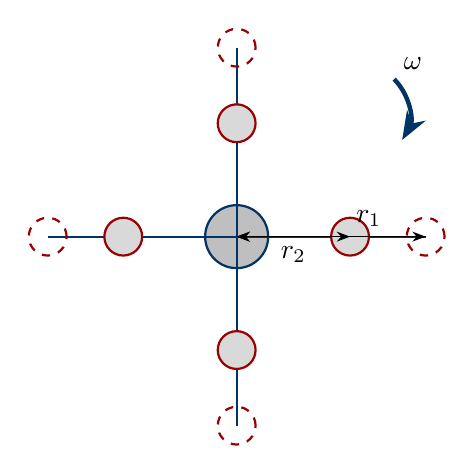
\begin{tikzpicture}[scale=0.8,>=Stealth]
    % Hub
    \draw[thick,examblue,fill=gray!50] (0,0) circle (0.5);
    
    % Spokes
    \foreach \a in {0,90,180,270}
        \draw[thick,examblue] (0,0)--(\a:3);
    
    % Masses (initial position - dashed)
    \foreach \a in {0,90,180,270}
        \draw[examred,dashed,thick] (\a:3) circle (0.3);
    
    % Masses (final position)
    \foreach \a in {0,90,180,270}
        \draw[examred,thick,fill=gray!30] (\a:1.8) circle (0.3);
    
    % Rotation
    \draw[->,examblue,ultra thick] (2.5,2.5) arc (45:-30:0.8);
    \node[above right] at (2.5,2.5) {$\omega$};
    
    % Labels
    \draw[<->] (0,0)--node[above,pos=0.7]{$r_1$}(0:3);
    \draw[<->] (0,0)--node[below,pos=0.5]{$r_2$}(0:1.8);
\end{tikzpicture}
\end{center}

Neglecting the hub inertia, determine the final angular velocity $\omega_2$.

\begin{mcqbox}
\begin{enumerate}[label=(\Alph*),leftmargin=*]
    \item $412\,\text{rpm}$
    \item $378\,\text{rpm}$
    \item $445\,\text{rpm}$
    \item $356\,\text{rpm}$
    \item $398\,\text{rpm}$
\end{enumerate}
\end{mcqbox}
\end{questionbox}

\begin{questionbox}
\subsection*{Question A5: Plastic Collapse of Continuous Beams [10 marks]}

The two-span continuous beam ABC has span $AB = 7\,\text{m}$ and $BC = 5\,\text{m}$. 
Span AB carries UDL $w_1 = 45\,\text{kN/m}$ and span BC has central point load $P = 180\,\text{kN}$.
The plastic moment capacity is $M_p = 280\,\text{kNm}$ for span AB and $1.5M_p$ for span BC.

\begin{center}
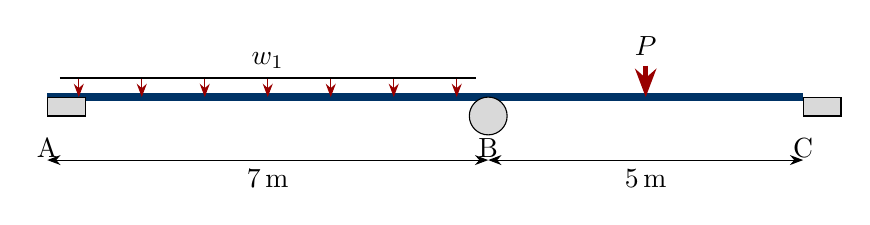
\begin{tikzpicture}[scale=0.8,>=Stealth]
    % Beam
    \draw[thick,examblue,line width=3pt] (0,0)--(7,0)--(12,0);
    
    % Supports
    \draw[fill=gray!30] (0,-0.3) rectangle ++(0.6,0.3);
    \draw[fill=gray!30] (7,-0.3) circle (0.3);
    \draw[fill=gray!30] (12,-0.3) rectangle ++(0.6,0.3);
    
    % UDL on AB
    \foreach \x in {0.5,1.5,...,6.5}
        \draw[->,examred] (\x,0.3)--(\x,0);
    \draw[thick] (0.2,0.3)--(6.8,0.3);
    \node[above] at (3.5,0.3) {$w_1$};
    
    % Point load on BC
    \draw[->,examred,ultra thick] (9.5,0.5)--(9.5,0);
    \node[above] at (9.5,0.5) {$P$};
    
    % Dimensions
    \draw[<->] (0,-1)--node[below]{$7\,\text{m}$}(7,-1);
    \draw[<->] (7,-1)--node[below]{$5\,\text{m}$}(12,-1);
    
    % Labels
    \node[below] at (0,-0.5) {A};
    \node[below] at (7,-0.5) {B};
    \node[below] at (12,-0.5) {C};
\end{tikzpicture}
\end{center}

Using plastic analysis and considering all possible collapse mechanisms, determine 
the load factor $\lambda$ at collapse.

\begin{mcqbox}
\begin{enumerate}[label=(\Alph*),leftmargin=*]
    \item $\lambda = 1.47$
    \item $\lambda = 1.63$
    \item $\lambda = 1.28$
    \item $\lambda = 1.85$
    \item $\lambda = 1.52$
\end{enumerate}
\end{mcqbox}
\end{questionbox}

\begin{questionbox}
\subsection*{Question A6: Vibration of Damped Systems [10 marks]}

A machine of mass $m = 450\,\text{kg}$ is mounted on springs with total stiffness 
$k = 280\,\text{kN/m}$ and a viscous damper. When displaced and released, the amplitude 
decays to 15\% of its initial value after 4 complete cycles.

\begin{center}
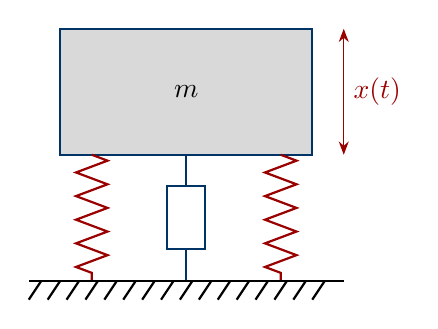
\begin{tikzpicture}[scale=0.8,>=Stealth]
    % Mass
    \draw[thick,examblue,fill=gray!30] (0,0) rectangle (4,2);
    \node at (2,1) {$m$};
    
    % Springs
    \draw[thick,examred,decorate,decoration={zigzag,segment length=3mm,amplitude=2mm}] 
        (0.5,0)--(0.5,-2);
    \draw[thick,examred,decorate,decoration={zigzag,segment length=3mm,amplitude=2mm}] 
        (3.5,0)--(3.5,-2);
    
    % Damper
    \draw[thick,examblue] (2,0)--(2,-0.5);
    \draw[thick,examblue] (1.7,-0.5) rectangle (2.3,-1.5);
    \draw[thick,examblue] (2,-1.5)--(2,-2);
    
    % Ground
    \draw[thick] (-0.5,-2)--(4.5,-2);
    \foreach \x in {-0.3,0,...,4.3}
        \draw[thick] (\x,-2)--++(-0.2,-0.3);
    
    % Displacement
    \draw[<->,examred] (4.5,0)--node[right]{$x(t)$}(4.5,2);
\end{tikzpicture}
\end{center}

Determine the damping ratio $\zeta$ and the damped natural frequency $\omega_d$.

\begin{mcqbox}
\begin{enumerate}[label=(\Alph*),leftmargin=*]
    \item $\zeta = 0.062$, $\omega_d = 24.7\,\text{rad/s}$
    \item $\zeta = 0.078$, $\omega_d = 24.9\,\text{rad/s}$
    \item $\zeta = 0.055$, $\omega_d = 24.5\,\text{rad/s}$
    \item $\zeta = 0.071$, $\omega_d = 24.8\,\text{rad/s}$
    \item $\zeta = 0.065$, $\omega_d = 24.6\,\text{rad/s}$
\end{enumerate}
\end{mcqbox}
\end{questionbox}

\newpage
\section*{SECTION B: LONG MULTIPLE CHOICE QUESTIONS (40 Marks)}
{\large\itshape Answer both questions. Each question carries 20 marks.}

\vspace{0.5cm}

\begin{questionbox}
\subsection*{Question B1: Matrix Stiffness Analysis of 3D Frame [20 marks]}

The space frame ABCD is fixed at A and D. Joint B carries loads $F_x = 20\,\text{kN}$, 
$F_y = -35\,\text{kN}$, $F_z = 15\,\text{kN}$. All members have circular hollow sections 
with $E = 200\,\text{GPa}$, $G = 77\,\text{GPa}$, $A = 4200\,\text{mm}^2$, 
$I = 28\times10^6\,\text{mm}^4$, $J = 52\times10^6\,\text{mm}^4$.

Coordinates: A(0,0,0), B(0,0,4), C(5,0,4), D(5,3,0) in meters.

\begin{center}
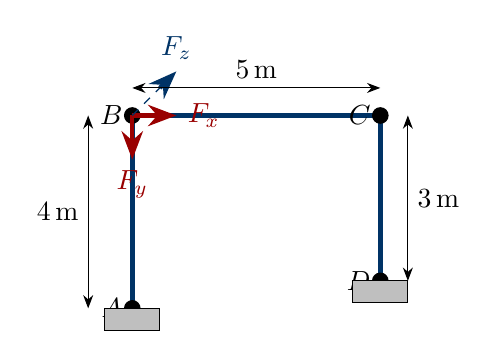
\begin{tikzpicture}[scale=0.7,>=Stealth]
    % 3D perspective
    \coordinate (A) at (0,0);
    \coordinate (B) at (0,3.5);
    \coordinate (C) at (4.5,3.5);
    \coordinate (D) at (4.5,0.5);
    
    % Members
    \draw[thick,examblue,line width=2pt] (A)--(B)--(C)--(D);
    
    % Joints
    \foreach \pt/\lbl in {A/A,B/B,C/C,D/D}
        \filldraw[black] (\pt) circle (4pt) node[left] {$\lbl$};
    
    % Fixed supports
    \draw[fill=gray!50] (A)++(-0.5,-0.4) rectangle ++(1,0.4);
    \draw[fill=gray!50] (D)++(-0.5,-0.4) rectangle ++(1,0.4);
    
    % Loads at B
    \draw[->,examred,ultra thick] (B)--++(0.8,0) node[right] {$F_x$};
    \draw[->,examred,ultra thick] (B)--++(0,-0.8) node[below] {$F_y$};
    \draw[examblue,dashed] (B)--++(0.5,0.5);
    \draw[->,examblue,ultra thick] (B)++(0.5,0.5)--++(0.3,0.3) node[above] {$F_z$};
    
    % Dimensions
    \draw[<->] (-0.8,0)--node[left]{$4\,\text{m}$}(-0.8,3.5);
    \draw[<->] (0,4)--node[above]{$5\,\text{m}$}(4.5,4);
    \draw[<->] (5,0.5)--node[right]{$3\,\text{m}$}(5,3.5);
\end{tikzpicture}
\end{center}

Using the matrix stiffness method with full 6 DOF per node, determine the vertical 
deflection at joint C.

\begin{mcqbox}
\begin{enumerate}[label=(\Alph*),leftmargin=*]
    \item $8.47\,\text{mm}$ downward
    \item $9.23\,\text{mm}$ downward
    \item $7.85\,\text{mm}$ downward
    \item $10.1\,\text{mm}$ downward
    \item $8.91\,\text{mm}$ downward
\end{enumerate}
\end{mcqbox}
\end{questionbox}

\begin{questionbox}
\subsection*{Question B2: Fracture Mechanics and Failure Assessment [20 marks]}

A pressure vessel (diameter $D = 1.8\,\text{m}$, wall thickness $t = 25\,\text{mm}$) contains 
a semi-elliptical surface crack with depth $a = 8\,\text{mm}$ and surface length $2c = 40\,\text{mm}$.
The vessel operates at internal pressure $p = 3.5\,\text{MPa}$ with superimposed cyclic thermal 
stress range $\Delta\sigma_{thermal} = 85\,\text{MPa}$.

Material properties: $K_{IC} = 95\,\text{MPa}\sqrt{\text{m}}$, 
$\frac{da}{dN} = C(\Delta K)^m$ where $C = 2.5\times10^{-12}$, $m = 3.2$.

Geometry factor for the crack: $Y = 1.12 + 0.23(a/c) - 0.11(a/c)^2$.

\begin{center}
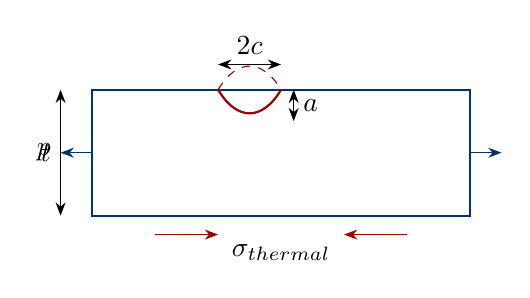
\begin{tikzpicture}[scale=0.8,>=Stealth]
    % Vessel wall section
    \draw[thick,examblue] (0,0) rectangle (6,2);
    
    % Crack
    \draw[examred,thick] (2,2)..controls(2.3,1.5)and(2.7,1.5)..(3,2);
    \draw[examred,dashed] (2,2)..controls(2.3,2.5)and(2.7,2.5)..(3,2);
    
    % Dimensions
    \draw[<->] (-0.5,0)--node[left]{$t$}(-0.5,2);
    \draw[<->] (2,2.4)--node[above]{$2c$}(3,2.4);
    \draw[<->] (3.2,2)--node[right]{$a$}(3.2,1.5);
    
    % Pressure
    \draw[->,examblue] (0,1)--(-0.5,1);
    \draw[->,examblue] (6,1)--(6.5,1);
    \node[left] at (-0.5,1) {$p$};
    
    % Thermal stress
    \draw[->,examred] (1,-0.3)--(2,-0.3);
    \draw[->,examred] (5,-0.3)--(4,-0.3);
    \node[below] at (3,-0.3) {$\sigma_{thermal}$};
\end{tikzpicture}
\end{center}

Using the Failure Assessment Diagram (FAD) approach and Paris law for crack growth, 
determine the number of cycles to failure.

\begin{mcqbox}
\begin{enumerate}[label=(\Alph*),leftmargin=*]
    \item $N_f = 47,500$ cycles
    \item $N_f = 52,300$ cycles
    \item $N_f = 41,800$ cycles
    \item $N_f = 58,900$ cycles
    \item $N_f = 45,200$ cycles
\end{enumerate}
\end{mcqbox}
\end{questionbox}

\end{document}
